\oldpage{412}\booktitle{Cincinnati Medical Observer}. Whether refusing to \emph{exchange} will
satisfy the profession that the charges made in the \booktitle{Observer} are without
foundation---are \emph{malicious} and \emph{false}, I cannot tell. The charge of falsehood
and malice must rest against the \booktitle{Observer} and its correspondent
if anywhere, for my remarks as I have shown are almost a literal quotation
from its pages.

\begin{figure}[H]
  \centering
  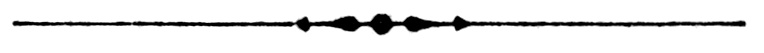
\includegraphics{pages/illustrations/arrow_bullet_divider.jpg}
\end{figure}

\section*{Tincture of Gelseminum in Dysentery.}

\byline*{\ProperName{H.~M.\ Kaigler}, \md}

\SectionStartWords{Being} favorably impressed with the medical properties of the Yellow
Jessamine, from what I read concerning its uses in various diseases by
Dr.\ Mayes, of South Carolina, I give you these few lines to know of
you in what diseases you have used it most. Dr.\ Mayes made frequent
mention of you in writing the article. I used it in one case and it answered
my expectations beyond my most sanguine hopes. It was a case
of dysentery in which the pulse ranged from one hundred and forty to
one hundred and sixty; in twelve hours time the pulse fell to one hundred
and two beats. I gave it because I was fearful that if I gave the
veratrum it would in all probability give rise to cartharsis in my almost
exhausted patient. It was the first time I had ever given the Tine, of
Jessamine; its effects were those as described by Dr.\ Mayes, viz: dimness
of vision, double-sightedness, inability to open the eye-lids, etc.

I at first gave twenty drops every three hours, afterwards increased it
to forty drops because of her dangerous situation. I prepared my tincture
according to the formula of Dr.\ Mayes; he put four ounces of the
root chopped fine in a pint of dilute alcohol and let it stand fourteen days;
he says from twenty to fifty drops is a dose. From his mentioning your
name as using the article largely in diseases, I address you to know
what is your manner of administering the medicine and in what diseases
do you think it will answer? Do you think it a remedy that will
cure Gonorrhea? Dr.\ Douglas of Chester, S.~C., says it will cure the above
named disease; he says he saw it used thirty years ago in that complaint.
I should like it very much if you would give me your views concerning
the article. We want something that will control the vascular system
without running any risk to our patient, as is frequently the case in
using the Tincture of Veratrum. The people in this part of the country
are so prejudiced against it that it is impossible to use it here, so we will
have to hunt up another remedy to use in its place.\endinput
